% MAS-FRO Defense Presentation (Beamer)
% Theme: Singapore
% Note: Compile with lualatex/xelatex or pdflatex (TikZ + listings required)
\documentclass[aspectratio=169]{beamer}
\usetheme{Singapore}
\usecolortheme{default}

% Packages
\usepackage{tikz}
\usetikzlibrary{arrows,positioning,shapes,calc,backgrounds}
\usepackage{listings}
\usepackage{amsmath,amssymb}
\usepackage{booktabs}
\usepackage{graphicx}
\usepackage{xcolor}
\usepackage{hyperref}
\hypersetup{colorlinks=true,linkcolor=blue,urlcolor=blue}

% Colors
\definecolor{darkgreen}{RGB}{0,100,0}
\definecolor{darkorange}{RGB}{255,140,0}
\definecolor{darkred}{RGB}{139,0,0}

% Code listings style
\lstdefinelanguage{json}{
  basicstyle=\ttfamily\footnotesize,
  showstringspaces=false,
  breaklines=true,
  literate=
   *{0}{{{\color{black}0}}}{1}
    {1}{{{\color{black}1}}}{1}
    {2}{{{\color{black}2}}}{1}
    {3}{{{\color{black}3}}}{1}
    {4}{{{\color{black}4}}}{1}
    {5}{{{\color{black}5}}}{1}
    {6}{{{\color{black}6}}}{1}
    {7}{{{\color{black}7}}}{1}
    {8}{{{\color{black}8}}}{1}
    {9}{{{\color{black}9}}}{1}
}
\lstset{
  language=Python,
  basicstyle=\footnotesize\ttfamily,
  keywordstyle=\color{blue},
  commentstyle=\color{gray},
  stringstyle=\color{red},
  numbers=left,
  numberstyle=\tiny,
  breaklines=true,
  frame=single
}

% Title page info
\title{MAS-FRO: Multi-Agent System for Flood Route Optimization}
\subtitle{Real-Time Flood-Safe Navigation for Marikina City, Philippines}
\author{[Student Name]}
\institute{De La Salle University \\ College of Computer Studies}
\date{November 2025}

\begin{document}

% -------------------------
% Title
% -------------------------
\begin{frame}
  \titlepage
  \vspace{-6pt}
  \begin{center}\small Prototype System (85\% Complete) --- Pending Comparative Validation\end{center}
\end{frame}

% -------------------------
% Problem & Motivation (6)
% -------------------------
\begin{frame}{The Ondoy Disaster (2009)}
  \begin{itemize}
    \item 455mm rainfall in 6 hours; 21.5m peak water level (\(\approx\)4.5m above critical)
    \item 464 deaths nationwide, 80+ in Marikina; PHP 11B damages
    \item Traditional navigation failed; residents routed into trap zones
  \end{itemize}
  \vspace{6pt}
  \begin{center}
  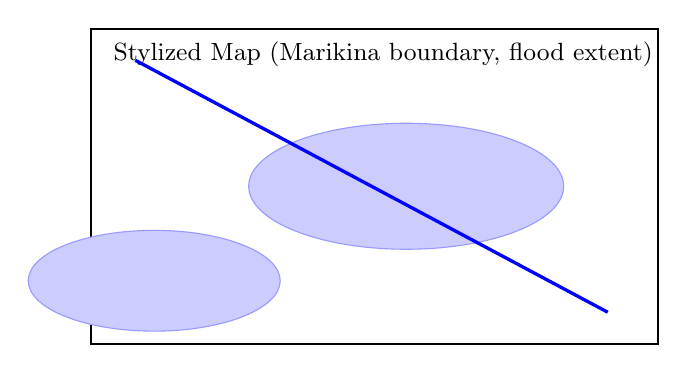
\begin{tikzpicture}[scale=0.8]
    \draw[thick] (0,0) rectangle (9,5);
    \node[anchor=west] at (0.2,4.6) {\small Stylized Map (Marikina boundary, flood extent)};
    \draw[fill=blue!20,draw=blue!40] (1,1) ellipse (2 and 0.8);
    \draw[fill=blue!20,draw=blue!40] (5,2.5) ellipse (2.5 and 1);
    \draw[very thick,blue] (0.7,4.5) -- (8.2,0.5);
  \end{tikzpicture}
  \end{center}
\end{frame}

\begin{frame}{Research Gap}
  \small
  \begin{tabular}{lccccc}
    \toprule
    System & Multi-Agent & Real-Time Flood & Crowdsourced & Risk-Aware & Deployed \\
    \midrule
    MAS-FRO & \(\checkmark\) & \(\checkmark\) & \(\checkmark\) & \(\checkmark\) & Prototype \\
    Google Maps & \(\times\) & \(\times\) & \(\checkmark\) (traffic) & \(\times\) & \(\checkmark\) \\
    DOST-NOAH & \(\times\) & \(\checkmark\) & \(\times\) & \(\times\) (monitor) & \(\checkmark\) \\
    Academic MAS & \(\checkmark\) & \(\times\) & \(\times\) & \(\times\) & \(\times\) (sim) \\
    \bottomrule
  \end{tabular}
  \vspace{6pt}
  \begin{block}{Conclusion}
    No existing system combines all four capabilities in an operational prototype.
  \end{block}
\end{frame}

\begin{frame}{Marikina City Context}
  \small
  \begin{itemize}
    \item Boundary: 21.5 km\(^2\); Population: \(\sim\)450,000
    \item Road network: \(|V|\approx 2{,}500\), \(|E|\approx 5{,}000\)
    \item Geographic extent: 14.61–14.75°N, 121.08–121.13°E
  \end{itemize}
  \vspace{4pt}
  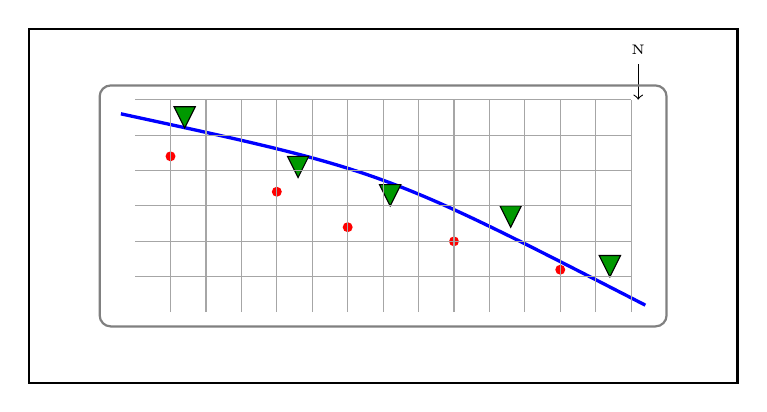
\begin{tikzpicture}[scale=0.9]
    \draw[thick] (0,0) rectangle (10,5);
    \node at (8.6,4.7) {\tiny N};
    \draw[->] (8.6,4.5)--(8.6,4.0);
    \draw[thick,rounded corners,gray] (1,0.8) rectangle (9,4.2);
    \draw[very thick,blue] (1.3,3.8) .. controls (5,3) .. (8.7,1.1);
    \foreach \x/\y in {2/3.2,3.5/2.7,4.5/2.2,6/2.0,7.5/1.6}{
      \fill[red] (\x,\y) circle (2pt);
    }
    \foreach \x/\y in {2.2/3.6,3.8/2.9,5.1/2.5,6.8/2.2,8.2/1.5}{
      \draw[fill=green!60!black] (\x,\y) -- +(0.15,0.3) -- +(-0.15,0.3) -- cycle;
    }
    \draw[gray!70] (1.5,1) grid[step=0.5] (8.5,4);
  \end{tikzpicture}
\end{frame}

\begin{frame}{Five Challenges}
  \begin{enumerate}
    \item Dynamic hazards: flood depth changes in minutes
    \item Multi-source data: PAGASA + OpenWeatherMap + GeoTIFF + Twitter/X
    \item Real-time performance: \(<2\)s route computation
    \item Data reliability: official sparse; crowdsourced noisy
    \item 24/7 availability: graceful degradation when APIs fail
  \end{enumerate}
\end{frame}

\begin{frame}{Research Objectives}
  \begin{itemize}
    \item Primary: Real-time flood-safe routing for Marikina City
    \item Specific aims:
    \begin{enumerate}
      \item Design hierarchical MAS (FIPA-ACL)
      \item Integrate real-time data sources (PAGASA, OWM, GeoTIFF)
      \item Implement risk-aware A* pathfinding
      \item Develop web prototype (Next.js + FastAPI)
      \item Validate performance (\alert{pending} comparative evaluation)
    \end{enumerate}
  \end{itemize}
\end{frame}

\begin{frame}{Scope \& Limitations (Upfront Honesty)}
  \small
  \begin{columns}[T,onlytextwidth]
    \column{0.33\textwidth}
      \textbf{In Scope}
      \begin{itemize}\itemsep2pt
        \item Marikina City only
        \item 5+ months operational
        \item Real APIs integrated
      \end{itemize}
    \column{0.33\textwidth}
      \textbf{Out of Scope}
      \begin{itemize}\itemsep2pt
        \item Other cities
        \item Multi-hazard
        \item Offline mode
      \end{itemize}
    \column{0.33\textwidth}
      \textbf{Validation Gaps}
      \begin{itemize}\itemsep2pt
        \item No baseline
        \item No real emergency deployment
        \item Expert validation pending
      \end{itemize}
  \end{columns}
\end{frame}

% -------------------------
% Theory (4)
% -------------------------
\begin{frame}{Multi-Agent Systems Theory}
  \small
  \begin{itemize}
    \item Wooldridge (1995): autonomy, reactivity, proactivity, social ability
  \end{itemize}
  \vspace{6pt}
  \begin{tabular}{lccc}
    \toprule
    Property & FloodAgent & HazardAgent & RoutingAgent \\
    \midrule
    Autonomy & \(\checkmark\) (5-min) & \(\checkmark\) (fusion) & \(\checkmark\) (on-demand) \\
    Reactivity & \(\checkmark\) & \(\checkmark\) & \(\checkmark\) \\
    Proactivity & \(\checkmark\) & \(\checkmark\) & \(\checkmark\) \\
    Social Ability & \(\checkmark\) (INFORM) & \(\checkmark\) & \(\checkmark\) (REQUEST/CONFIRM) \\
    \bottomrule
  \end{tabular}
  \vspace{6pt}
  \begin{block}{FIPA-ACL}
    Standard performatives for agent communication (REQUEST, INFORM, CONFIRM, \dots)
  \end{block}
\end{frame}

\begin{frame}{Graph Theory \& A* Algorithm}
  \small
  \begin{itemize}
    \item Road network: directed multi-graph \(G=(V,E,W)\), \(|V|\approx 2{,}500\), \(|E|\approx 5{,}000\)
    \item A*: \(f(n)=g(n)+h(n)\). If \(h\) admissible \(\Rightarrow\) optimal path
    \item Haversine heuristic; Complexity: \(\mathcal{O}((|V|+|E|)\log |V|)\)
  \end{itemize}
  \vspace{6pt}
  \begin{block}{Heuristic}
    Great-circle approximation sufficient at Marikina scale (\(<50\)m error typical).
  \end{block}
\end{frame}

\begin{frame}{Risk Assessment \& MCDM}
  \small
  \begin{itemize}
    \item Weighted sum: \( \text{Cost} = w_d \cdot \text{distance} + w_r \cdot \text{risk} \)
    \item Current weights: \(w_d=0.4\), \(w_r=0.6\) (\emph{heuristic}; to be calibrated)
  \end{itemize}
  \vspace{6pt}
  \begin{block}{Passability Constraint}
    If \(r(e)\ge 0.9\Rightarrow C(e)=\infty\) (edge blocked).
  \end{block}
\end{frame}

\begin{frame}{Data Fusion (Terminology Correction)}
  \small
  \textbf{Simplified Bayesian-Inspired Weighted Aggregation}
  \[
    R_{\text{fused}}=\alpha_1 R_{\text{official}}+\alpha_2 R_{\text{crowd}}+\alpha_3 R_{\text{hist}}
  \]
  \(\alpha_1=0.5, \alpha_2=0.3, \alpha_3=0.2\)
  \begin{block}{Note}
    Weighted averaging, not full Bayesian inference. Future work: full Bayesian model with priors and likelihoods.
  \end{block}
\end{frame}

% -------------------------
% Related Work (3)
% -------------------------
\begin{frame}{Related Work - Categories}
  \small
  \begin{enumerate}\itemsep4pt
    \item Disaster routing (offline planning)
    \item Commercial navigation (no flood awareness)
    \item Government monitoring (no routing)
    \item Multi-agent simulation (not deployed)
    \item Philippine systems (monitoring only)
  \end{enumerate}
  \vspace{4pt}
  \alert{Gap:} No paper/system combines MAS + real-time flood + operational prototype.
\end{frame}

\begin{frame}{Risk-Aware Pathfinding Timeline}
  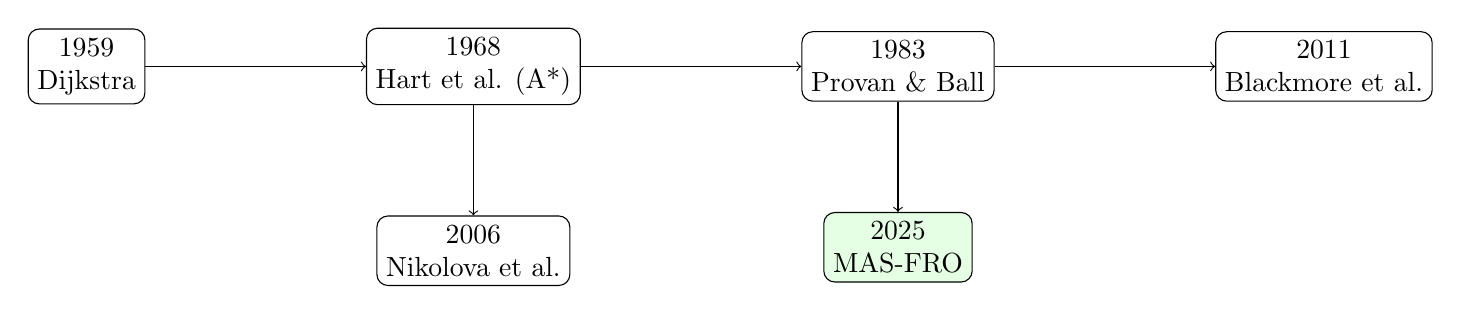
\begin{tikzpicture}[node distance=1.7cm]
    \node (n1) [draw,rounded corners,align=center] {1959\\Dijkstra};
    \node (n2) [draw,rounded corners,align=center,right=2.8cm of n1] {1968\\Hart et al. (A*)};
    \node (n3) [draw,rounded corners,align=center,right=2.8cm of n2] {1983\\Provan \& Ball};
    \node (n4) [draw,rounded corners,align=center,below=1.4cm of n2] {2006\\Nikolova et al.};
    \node (n5) [draw,rounded corners,align=center,right=2.8cm of n3] {2011\\Blackmore et al.};
    \node (n6) [draw,rounded corners,align=center,below=1.4cm of n3,fill=green!10] {2025\\MAS-FRO};
    \draw[->] (n1)--(n2);
    \draw[->] (n2)--(n3);
    \draw[->] (n3)--(n5);
    \draw[->] (n2)--(n4);
    \draw[->] (n3)--(n6);
  \end{tikzpicture}
  \vspace{6pt}
  \begin{center}\small Application of established techniques to a novel operational domain.\end{center}
\end{frame}

\begin{frame}{MAS-FRO Unique Niche}
  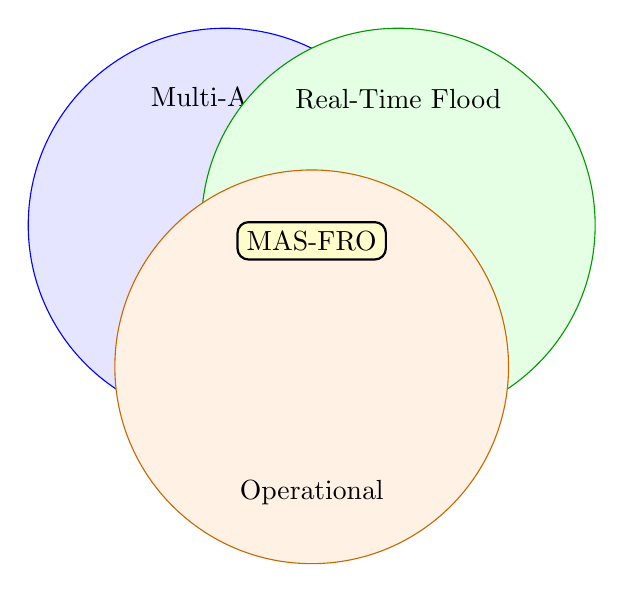
\begin{tikzpicture}
    \def\r{2.5}
    \begin{scope}[shift={(0,0)}]
      \draw[fill=blue!10,draw=blue] (0,0) circle (\r);
      \node at (0,1.6) {Multi-Agent};
    \end{scope}
    \begin{scope}[shift={(2.2,0)}]
      \draw[fill=green!10,draw=green!60!black] (0,0) circle (\r);
      \node at (0,1.6) {Real-Time Flood};
    \end{scope}
    \begin{scope}[shift={(1.1,-1.8)}]
      \draw[fill=orange!10,draw=orange!80!black] (0,0) circle (\r);
      \node at (0,-1.6) {Operational};
    \end{scope}
    \node[draw,thick,fill=yellow!20,rounded corners] at (1.1,-0.2) {MAS-FRO};
  \end{tikzpicture}
  \vspace{4pt}
  \small Others: Google Maps (Real-time+Operational), RoboCup (MAS), NOAH (Real-time).
\end{frame}

% -------------------------
% System Architecture (10)
% -------------------------
\begin{frame}{Architecture Overview}
  \begin{center}
  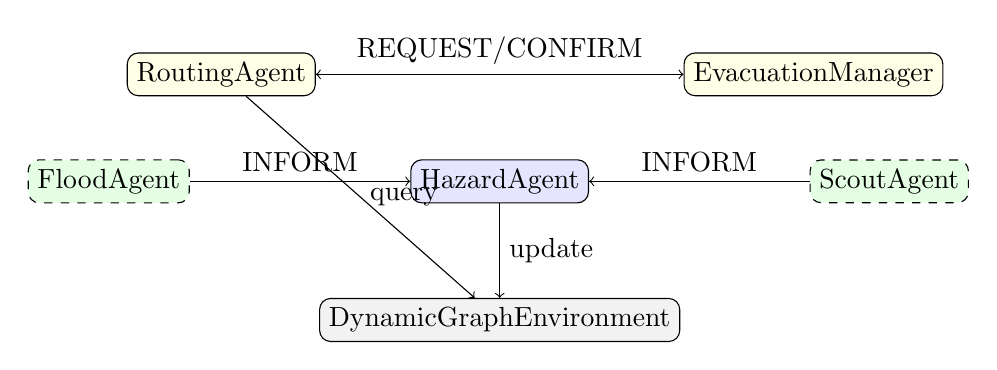
\begin{tikzpicture}[node distance=1.2cm]
    \node[draw,rounded corners,fill=gray!10] (env) {DynamicGraphEnvironment};
    \node[draw,rounded corners,above=of env,fill=blue!10] (haz) {HazardAgent};
    \node[draw,dashed,rounded corners,left=2.8cm of haz,fill=green!10] (flood) {FloodAgent};
    \node[draw,dashed,rounded corners,right=2.8cm of haz,fill=green!10] (scout) {ScoutAgent};
    \node[draw,rounded corners,above left=0.8cm and 1.2cm of haz,fill=yellow!10] (route) {RoutingAgent};
    \node[draw,rounded corners,above right=0.8cm and 1.2cm of haz,fill=yellow!10] (evac) {EvacuationManager};
    \draw[->] (flood) -- node[above,sloped]{INFORM} (haz);
    \draw[->] (scout) -- node[above,sloped]{INFORM} (haz);
    \draw[->] (haz) -- node[right]{update} (env);
    \draw[<->] (route) -- node[above]{REQUEST/CONFIRM} (evac);
    \draw[->] (route) -- node[right]{query} (env);
  \end{tikzpicture}
  \end{center}
\end{frame}

\begin{frame}{Agent Roles Matrix}
  \small
  \begin{tabular}{llllll}
    \toprule
    Agent & Type & Role & LOC & File & Status \\
    \midrule
    FloodAgent & Collector & Official data (PAGASA, OWM) & 960 & \texttt{flood\_agent.py} & Operational \\
    ScoutAgent & Collector & Crowdsourced (Twitter/X NLP) & 486 & \texttt{scout\_agent.py} & Operational \\
    HazardAgent & Coordinator & Fusion, risk calculation & 594 & \texttt{hazard\_agent.py} & Operational \\
    RoutingAgent & Service & Risk-aware A* & 459 & \texttt{routing\_agent.py} & Operational \\
    EvacuationMgr & Interface & Requests, feedback & 430 & \texttt{evacuation\_manager\_agent.py} & Operational \\
    \bottomrule
  \end{tabular}
\end{frame}

\begin{frame}[fragile]{FIPA-ACL Message Example}
\begin{lstlisting}
ACLMessage(
    performative=Performative.INFORM,
    sender="flood_agent_001",
    receiver="hazard_agent_001",
    content={
        "info_type": "flood_data_update",
        "data": {
            "Sto Nino": {
                "water_level": 15.2,
                "risk_level": "ALERT"
            }
        }
    },
    conversation_id="collection_12345"
)
\end{lstlisting}
\end{frame}

\begin{frame}{Communication Sequence}
  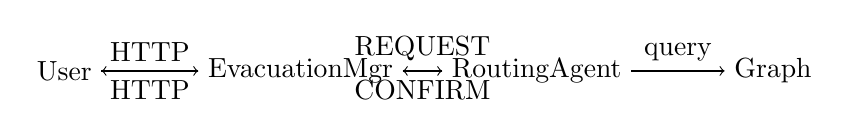
\begin{tikzpicture}[node distance=1.2cm]
    \node (user) at (0,0) {User};
    \node (evac) at (3,0) {EvacuationMgr};
    \node (route) at (6,0) {RoutingAgent};
    \node (graph) at (9,0) {Graph};
    \draw[->] (user) -- node[above]{HTTP} (evac);
    \draw[->] (evac) -- node[above]{REQUEST} (route);
    \draw[->] (route) -- node[above]{query} (graph);
    \draw[->] (route) -- node[below]{CONFIRM} (evac);
    \draw[->] (evac) -- node[below]{HTTP} (user);
  \end{tikzpicture}
  \vspace{6pt}
  \small T=0s to T=3s (typical).
\end{frame}

\begin{frame}{Dynamic Graph Environment}
  \small
  \begin{itemize}
    \item Edge weights: \(W(e,t)= \text{length}(e)\cdot r(e,t)\)
    \item Risk color map: green (low) \(\rightarrow\) red (high)
    \item Update cadence: 5 minutes
  \end{itemize}
  \vspace{6pt}
  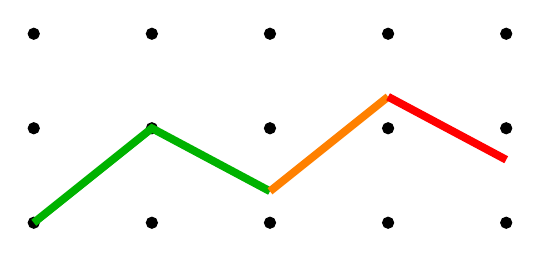
\begin{tikzpicture}
    \foreach \i in {0,...,4}{
      \foreach \j in {0,...,2}{
        \filldraw (0.8+1.5*\i,0.8+1.2*\j) circle (2pt);
      }
    }
    \draw[line width=1mm,green!70!black] (0.8,0.8)--(2.3,2.0)--(3.8,1.2);
    \draw[line width=1mm,orange] (3.8,1.2)--(5.3,2.4);
    \draw[line width=1mm,red] (5.3,2.4)--(6.8,1.6);
  \end{tikzpicture}
\end{frame}

\begin{frame}[fragile]{Risk-Aware A*: Balancing Safety and Distance}
  \begin{columns}[T,onlytextwidth]
    \column{0.52\textwidth}
      \small
      \( C(e) =
      \begin{cases}
        \infty & r(e)\ge 0.9 \\
        w_d \cdot d(e) + w_r \cdot d(e)\cdot r(e) & \text{otherwise}
      \end{cases}\)
      \vspace{8pt}

      \(\Rightarrow\) \(\text{Cost}(P)=\sum_{e\in P} C(e)\), minimize over all paths
    \column{0.46\textwidth}
\begin{lstlisting}
def weight_function(u, v, edge_data):
    length = edge_data['length']
    risk = edge_data['risk_score']
    if risk >= 0.9:
        return float('inf')
    return w_d * length + w_r * length * risk
\end{lstlisting}
  \end{columns}
\end{frame}

\begin{frame}{Multi-Source Data Fusion}
  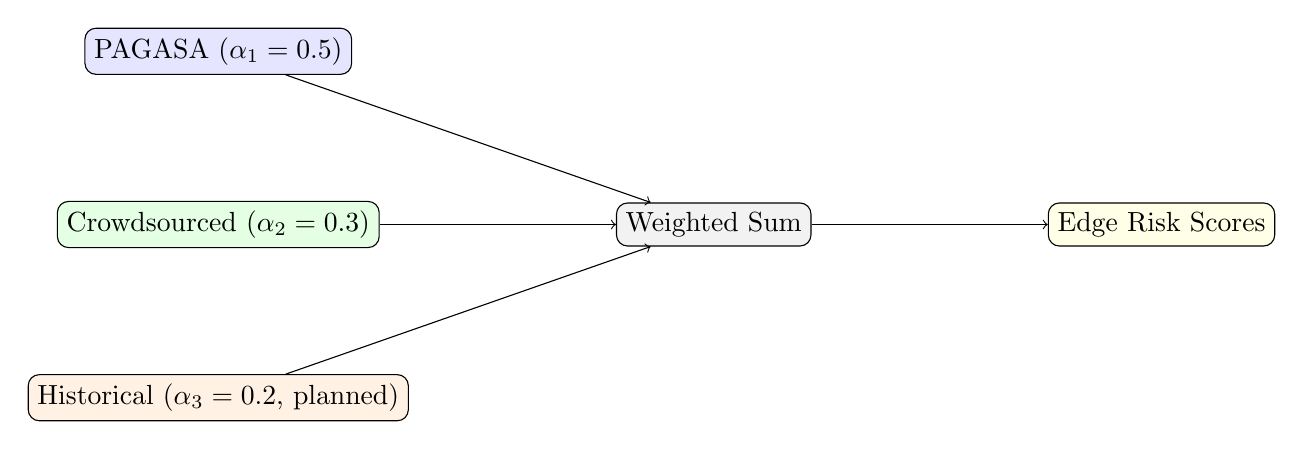
\begin{tikzpicture}[node distance=1.6cm]
    \node[draw,rounded corners,fill=blue!10] (p1) {PAGASA (\(\alpha_1=0.5\))};
    \node[draw,rounded corners,below=of p1,fill=green!10] (p2) {Crowdsourced (\(\alpha_2=0.3\))};
    \node[draw,rounded corners,below=of p2,fill=orange!10] (p3) {Historical (\(\alpha_3=0.2\), planned)};
    \node[draw,rounded corners,right=3.0cm of p2,fill=gray!10] (fuse) {Weighted Sum};
    \node[draw,rounded corners,right=3.0cm of fuse,fill=yellow!10] (out) {Edge Risk Scores};
    \draw[->] (p1)--(fuse);
    \draw[->] (p2)--(fuse);
    \draw[->] (p3)--(fuse);
    \draw[->] (fuse)--(out);
  \end{tikzpicture}
  \vspace{6pt}
  \alert{Weights heuristic; empirical calibration pending (publication gap).}
\end{frame}

\begin{frame}[fragile]{FloodAgent Implementation (Key Method)}
\begin{lstlisting}
def fetch_real_river_levels(self) -> Dict:
    """Fetch from PAGASA API, filter Marikina stations."""
    stations = self.river_scraper.get_river_levels()  # 17 stations
    marikina_stations = ["Sto Nino", "Nangka", "Tumana",
                         "Montalban", "Rosario Bridge"]
    filtered = {s['name']: classify_risk(s['water_level'],
                                         s['critical_level'])
                for s in stations if s['name'] in marikina_stations}
    return filtered  # 5 stations
\end{lstlisting}
\end{frame}

\begin{frame}[fragile]{HazardAgent Implementation (Fusion Logic)}
\begin{lstlisting}
def fuse_data(self) -> Dict[str, Any]:
    """Weighted multi-source aggregation."""
    fused = {}
    for edge in graph.edges():
        depth = geotiff.get_depth(edge_midpoint)  # official
        R_official = map_depth_to_risk(depth)
        reports = find_reports_within_500m(edge)  # crowd
        R_crowd = average_severity(reports)
        risk = 0.5*R_official + 0.3*R_crowd + 0.2*R_hist
        fused[edge] = min(risk, 1.0)
    return fused
\end{lstlisting}
\end{frame}

\begin{frame}{System Statistics}
  \begin{itemize}
    \item 5 Autonomous Agents; \(\sim\)8,000 LOC
    \item PAGASA stations: 17\(\rightarrow\)5 (Marikina-filtered)
    \item 72 GeoTIFF flood maps; \(|V|\approx 2{,}500\), \(|E|\approx 5{,}000\)
    \item Update cycle: 5 minutes; 95\% real data
  \end{itemize}
\end{frame}

% -------------------------
% Agreement Form Compliance (8)
% -------------------------
\begin{frame}{Agreement Form Overview}
  \small
  \begin{tabular}{llll}
    \toprule
    Item & Description & Status & Gap \\
    \midrule
    1 & MAS Communication & \textcolor{darkorange}{4/5} & Stress testing \\
    2 & Dynamic Graph & \textcolor{darkgreen}{5/5} & Calibration pending \\
    3 & Baseline & \textcolor{darkred}{0/3} & \textbf{CRITICAL} \\
    4 & Risk-Aware A* & \textcolor{darkgreen}{Complete} & -- \\
    5 & Simulation & \textcolor{darkorange}{2/4} & Systematic testing \\
    6 & Web Prototype & \textcolor{darkgreen}{Complete} & -- \\
    7 & Paper & \textcolor{darkred}{Rejected} & 3,5,1.v \\
    \bottomrule
  \end{tabular}
\end{frame}

\begin{frame}{Item 1 - MAS Communication (4/5)}
  \small
  \begin{itemize}
    \item \(\checkmark\) Roles defined (5 agents)
    \item \(\checkmark\) Middleware (FIPA-ACL)
    \item \(\checkmark\) Message formats (dataclass, 9 performatives)
    \item \(\triangle\) Failover: graceful degradation only
    \item \(\times\) Network stress testing (not conducted)
  \end{itemize}
  Evidence: \texttt{app/communication/acl\_protocol.py}, \texttt{message\_queue.py}
\end{frame}

\begin{frame}{Item 2 - Dynamic Graph (5/5)}
  \small
  \begin{itemize}
    \item \(\checkmark\) NetworkX MultiDiGraph; OSMnx (Marikina)
    \item \(\checkmark\) 72 GeoTIFF hazard maps
    \item \(\checkmark\) Real-time updates (5-min cadence)
    \item \(\checkmark\) Hazard scoring implemented (\emph{weights heuristic})
  \end{itemize}
  Caveat: Weight calibration pending.
\end{frame}

\begin{frame}{Item 3 - Baseline (\textcolor{darkred}{Critical Gap})}
  \small
  \begin{itemize}
    \item 0/3 complete: centralized baseline, time/accuracy/scalability comparisons absent
    \item Primary reason for paper rejection
    \item Roadmap: 16–20 hours to implement \& test
  \end{itemize}
\end{frame}

\begin{frame}{Item 4 - Risk-Aware A* (Complete)}
  \small
  \[
    P^*=\arg\min_{P\in\mathcal{P}(s,t)} \sum_{e\in P} C(e),\quad
    C(e)=
    \begin{cases}
      \infty & r(e)\ge 0.9\\
      w_d d(e)+ w_r d(e) r(e) & \text{otherwise}
    \end{cases}
  \]
  Complexity: \(\mathcal{O}((|V|+|E|)\log |V|)\).
\end{frame}

\begin{frame}{Item 5 - Simulation Testing (2/4)}
  \small
  \begin{itemize}
    \item \(\checkmark\) Agent instances configured
    \item \(\triangle\) Multi-scenario tests exist but not systematic
    \item \(\times\) Metrics collection (manual, \(n\approx 20\))
    \item \(\triangle\) Logs: stdout only
  \end{itemize}
  Gap: Framework + automation (20–24 hours).
\end{frame}

\begin{frame}{Item 6 - Web Prototype (Complete)}
  \small
  \begin{itemize}
    \item Next.js 15 + Mapbox GL; 18+ REST endpoints
    \item WebSocket (5-min updates); PostgreSQL (5+ months data)
    \item Status: Functional prototype (\emph{not} production-hardened)
  \end{itemize}
\end{frame}

\begin{frame}{Item 7 - Paper Status (Rejected)}
  \small
  Probable reasons:
  \begin{enumerate}
    \item No baseline comparison
    \item No systematic validation
    \item No stress testing
    \item Incomplete calibration
    \item Overstated novelty
  \end{enumerate}
  \vspace{4pt}
  Roadmap: Phase 1 (56–72h) to close 3,5,1.v; Phase 2: real-world validation.
\end{frame}

% -------------------------
% Implementation Highlights (5)
% -------------------------
\begin{frame}{Real-Time Data Integration}
  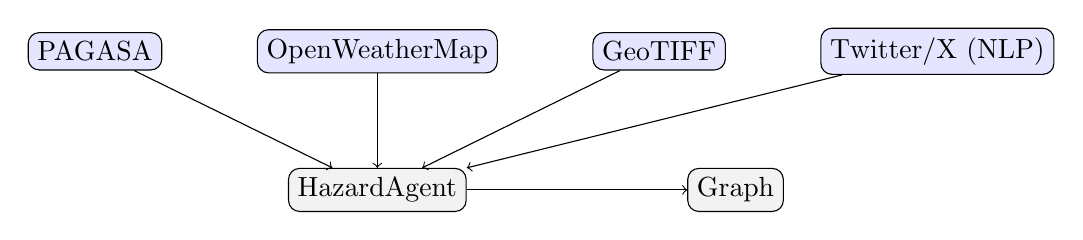
\begin{tikzpicture}[node distance=1.2cm]
    \node[draw,rounded corners,fill=blue!10] (p1) {PAGASA};
    \node[draw,rounded corners,right=of p1,fill=blue!10] (p2) {OpenWeatherMap};
    \node[draw,rounded corners,right=of p2,fill=blue!10] (p3) {GeoTIFF};
    \node[draw,rounded corners,right=of p3,fill=blue!10] (p4) {Twitter/X (NLP)};
    \node[draw,rounded corners,below=1.2cm of p2,fill=gray!10] (haz) {HazardAgent};
    \node[draw,rounded corners,right=2.8cm of haz,fill=gray!10] (graph) {Graph};
    \draw[->] (p1)--(haz);
    \draw[->] (p2)--(haz);
    \draw[->] (p3)--(haz);
    \draw[->] (p4)--(haz);
    \draw[->] (haz)--(graph);
  \end{tikzpicture}
  \vspace{6pt}
  Update cadence: 5 minutes. API costs: within free tier.
\end{frame}

\begin{frame}{GeoTIFF Service Architecture}
  \small
  \begin{enumerate}\itemsep2pt
    \item Select return period/time-step
    \item Lazy load \texttt{.tif}
    \item LRU cache (max 32)
    \item WGS84 \(\rightarrow\) Web Mercator
    \item Pixel lookup (e.g., 368\(\times\)372 raster)
    \item Return flood depth (m)
  \end{enumerate}
  \vspace{4pt}
  Performance: \(<0.1\)s/query with cache.
\end{frame}

\begin{frame}{WebSocket Real-Time Architecture}
  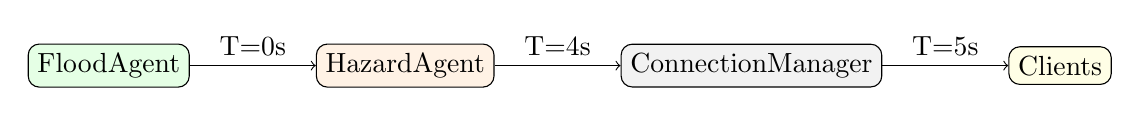
\begin{tikzpicture}[node distance=1.6cm]
    \node[draw,rounded corners,fill=green!10] (fa) {FloodAgent};
    \node[draw,rounded corners,fill=orange!10,right=of fa] (ha) {HazardAgent};
    \node[draw,rounded corners,fill=gray!10,right=of ha] (cm) {ConnectionManager};
    \node[draw,rounded corners,fill=yellow!10,right=of cm] (cli) {Clients};
    \draw[->] (fa)-- node[above]{T=0s} (ha);
    \draw[->] (ha)-- node[above]{T=4s} (cm);
    \draw[->] (cm)-- node[above]{T=5s} (cli);
  \end{tikzpicture}
  \vspace{4pt}
  Message types: \texttt{flood\_update}, \texttt{critical\_alert}, \texttt{scheduler\_update}.
\end{frame}

\begin{frame}{Database Schema (ER Diagram)}
  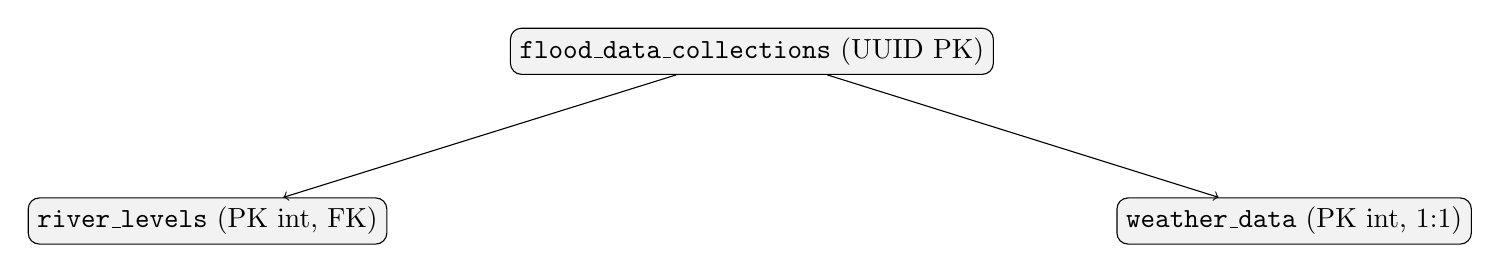
\begin{tikzpicture}[node distance=2.2cm]
    \node[draw,rounded corners,fill=gray!10] (c) {\texttt{flood\_data\_collections} (UUID PK)};
    \node[draw,rounded corners,fill=gray!10,below left=of c] (r) {\texttt{river\_levels} (PK int, FK)};
    \node[draw,rounded corners,fill=gray!10,below right=of c] (w) {\texttt{weather\_data} (PK int, 1:1)};
    \draw[->] (c)--(r);
    \draw[->] (c)--(w);
  \end{tikzpicture}
  \vspace{6pt}
  PostgreSQL 14+, SQLAlchemy 2.0, Alembic. 10,000+ records (5+ months).
\end{frame}

\begin{frame}{Dependency Overview}
  \small
  \begin{columns}[T,onlytextwidth]
    \column{0.48\textwidth}
      \textbf{Backend (Python)}
      \begin{itemize}\itemsep2pt
        \item FastAPI 0.118 (REST/WebSocket)
        \item NetworkX 3.4 (Graph)
        \item OSMnx 2.0 (OSM)
        \item Rasterio 1.4 (GeoTIFF)
        \item SQLAlchemy 2.0 (ORM)
        \item Selenium 4.36 (Scraping)
      \end{itemize}
    \column{0.48\textwidth}
      \textbf{Frontend (JavaScript)}
      \begin{itemize}\itemsep2pt
        \item Next.js 15.5 (React framework)
        \item Mapbox GL 3.15 (WebGL map)
        \item geotiff.js 2.1 (TIFF parsing)
        \item Tailwind CSS 4 (Styling)
      \end{itemize}
  \end{columns}
\end{frame}

% -------------------------
% Performance (3)
% -------------------------
\begin{frame}{Preliminary Performance Metrics}
  \small
  \begin{tabular}{llll}
    \toprule
    Metric & Observed & Method & Sample \\
    \midrule
    Route calc & 0.5–2s (\(\mu=1.2\)s, \(\sigma=0.4\)s) & Manual & \(n=20\) \\
    PAGASA API & 1–3s & requests & \(n=15\) \\
    OWM API & 0.5–1s & requests & \(n=15\) \\
    GeoTIFF & <0.1s & Rasterio+cache & \(n=100\) \\
    DB & <100ms & SQLAlchemy & \(n=50\) \\
    WebSocket & <50ms & AsyncIO & \(n=20\) \\
    \bottomrule
  \end{tabular}
  \vspace{4pt}
  \alert{Preliminary; systematic benchmarking not yet conducted.}
\end{frame}

\begin{frame}{System Operational Statistics}
  \small
  \begin{itemize}
    \item 5+ months operational; 10,000+ DB records
    \item 288 API calls/day (5-min intervals)
    \item 95\% real data success; 0 critical failures
  \end{itemize}
\end{frame}

\begin{frame}{Data Quality Assessment}
  \small
  \begin{itemize}
    \item 95\% real APIs, 5\% simulated fallback
    \item Source uptime: PAGASA 100\%, OWM 100\%, GeoTIFF local
  \end{itemize}
\end{frame}

% -------------------------
% Critical Assessment (5)
% -------------------------
\begin{frame}{Limitations (Academic Honesty)}
  \small
  \begin{itemize}\itemsep2pt
    \item Geographic: Marikina-only; no multi-city routing
    \item Validation: no baseline; no real emergency test; small sample; no expert study
    \item Algorithm: heuristic parameters; no uncertainty quantification
    \item Data sources: PAGASA reliability; OWM forecast accuracy; static GeoTIFF
    \item System: no formal failover; no load balancing; limited monitoring
    \item UX: desktop-first; no offline; English-only
  \end{itemize}
\end{frame}

\begin{frame}{Publication Gaps Analysis}
  \small
  \begin{columns}[T,onlytextwidth]
    \column{0.32\textwidth}
      \textbf{Complete}
      \begin{itemize}\itemsep2pt
        \item Dynamic graph
        \item Risk-aware A*
        \item Web prototype
      \end{itemize}
    \column{0.32\textwidth}
      \textbf{Partial}
      \begin{itemize}\itemsep2pt
        \item MAS communication (4/5)
        \item Simulation (2/4)
      \end{itemize}
    \column{0.32\textwidth}
      \textbf{Missing}
      \begin{itemize}\itemsep2pt
        \item Baseline
        \item Comparative evaluation
        \item Statistical validation
      \end{itemize}
  \end{columns}
\end{frame}

\begin{frame}{Roadmap to Q1-Ready}
  \small
  \begin{itemize}
    \item Short-Term (3–6 mo): baseline; systematic tests; stress tests; calibration (\(\sim\)56–72h eng effort)
    \item Medium-Term (6–12 mo): real-world validation; expert/user studies
    \item Publication (12–15 mo): revise paper; resubmit
  \end{itemize}
\end{frame}

\begin{frame}{Honest Assessment for Panel}
  \begin{quote}\small
    MAS-FRO is a functional prototype demonstrating feasibility of multi-agent flood routing. It represents strong graduate-level work. However, it lacks comparative evaluation and real-world validation required for Q1 journal publication. With gap closure and deployment, it will be publication-ready as an application/systems paper.
  \end{quote}
\end{frame}

\begin{frame}{Lessons Learned}
  \small
  \begin{enumerate}\itemsep2pt
    \item Implement baseline early (enable comparative evaluation)
    \item Automate systematic testing (avoid manual-only evidence)
    \item Qualify contributions (application vs algorithmic novelty)
    \item Calibrate parameters empirically
    \item Validate in real events (beyond simulation)
  \end{enumerate}
\end{frame}

% -------------------------
% Future Work & Conclusion (3)
% -------------------------
\begin{frame}{Research Contributions (Qualified)}
  \small
  \begin{tabular}{clll}
    \toprule
    \# & Contribution & Type & Evidence \\
    \midrule
    1 & Risk-Aware A* for PH floods & Domain Application & PAGASA + 5-min updates \\
    2 & Real-Time Multi-Source Aggregation & Engr. Framework & 4 sources; 95\% real data \\
    3 & FIPA-ACL for Disaster MAS & Standards Impl. & 9 performatives; queue \\
    4 & Functional Prototype (Gov APIs) & Systems Engr. & OWM + GeoTIFF operational \\
    \bottomrule
  \end{tabular}
\end{frame}

\begin{frame}{Future Work}
  \small
  \textbf{Phase 1} (Short-term): baseline, tests, calibration \(\Rightarrow\) pub-ready\\
  \textbf{Phase 2} (Medium-term): ML (RF/LSTM), Metro Manila, mobile app\\
  \textbf{Phase 3} (Long-term): true Bayesian fusion; multi-hazard; LGU integration
\end{frame}

\begin{frame}{Conclusion}
  \small
  \begin{columns}[T,onlytextwidth]
    \column{0.32\textwidth}
      \textbf{Achievements}
      \begin{itemize}\itemsep2pt
        \item 5-agent MAS (FIPA-ACL)
        \item Real gov APIs
        \item 72 GeoTIFF maps
        \item Functional prototype
        \item 5+ months operational
      \end{itemize}
    \column{0.32\textwidth}
      \textbf{Gaps}
      \begin{itemize}\itemsep2pt
        \item No baseline
        \item No systematic testing
        \item No stress testing
        \item Heuristic parameters
      \end{itemize}
    \column{0.32\textwidth}
      \textbf{Path Forward}
      \begin{itemize}\itemsep2pt
        \item 56–72h: close gaps
        \item 6–12mo: validation
        \item 12–15mo: Q1 submission
      \end{itemize}
  \end{columns}
\end{frame}

\begin{frame}{Questions?}
  \centering
  \Large Questions?\\[8pt]
  \normalsize Backup slides available for technical deep dives.
\end{frame}

% -------------------------
% Backup Slides (12)
% -------------------------
\appendix

\begin{frame}{A* Admissibility Proof (Sketch)}
  \small
  \textbf{Claim:} Haversine distance is admissible \(\Rightarrow\) never overestimates geodesic distance.\\[4pt]
  \textbf{Sketch:} Great-circle distance lower bounds path along road network; therefore \(h(n)\le h^*(n)\).
\end{frame}

\begin{frame}{Complexity Derivation (Detailed)}
  \small
  Binary heap priority queue: insert/extract \(\mathcal{O}(\log |V|)\); each edge scanned once \(\Rightarrow \mathcal{O}((|V|+|E|)\log |V|)\).
\end{frame}

\begin{frame}[fragile]{Risk Calculation Code (Complete Example)}
\begin{lstlisting}
def calculate_risk_scores(self, fused_data: Dict) -> Dict:
    risk_scores = {}
    for u, v, key in self.environment.graph.edges():
        edge_data = self.environment.graph[u][v][key]
        geometry = edge_data.get('geometry')
        if not geometry:
            continue
        midpoint = geometry.interpolate(0.5, normalized=True)
        depth = self.geotiff_service.get_flood_depth_at_point(
            midpoint.x, midpoint.y, self.return_period, self.time_step
        )
        depth_risk = self._map_depth_to_risk(depth)
        prox_risk = self._calculate_proximity_risk(geometry, fused_data)
        combined = 0.6 * depth_risk + 0.4 * prox_risk
        risk_scores[(u, v, key)] = min(combined, 1.0)
    return risk_scores
\end{lstlisting}
\end{frame}

\begin{frame}{Database Schema (Full ER Sketch)}
  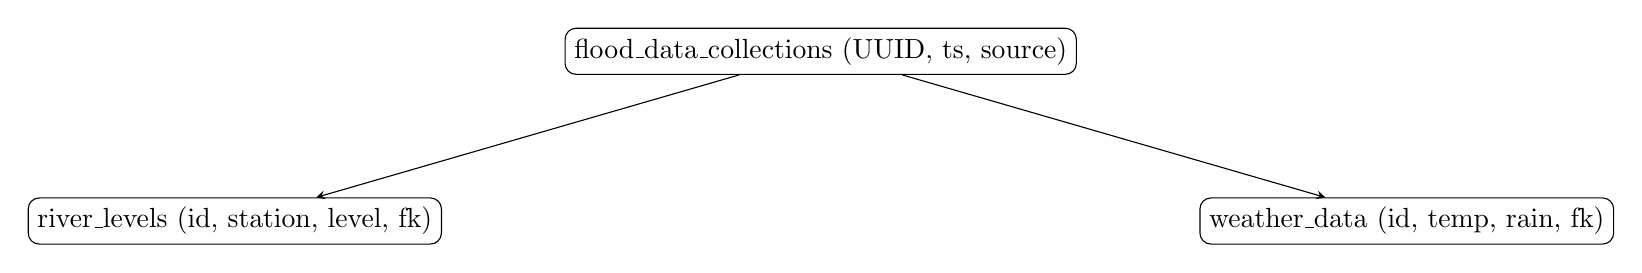
\begin{tikzpicture}[node distance=2.2cm]
    \node[draw,rounded corners] (c) {flood\_data\_collections (UUID, ts, source)};
    \node[draw,rounded corners,below left=of c] (r) {river\_levels (id, station, level, fk)};
    \node[draw,rounded corners,below right=of c] (w) {weather\_data (id, temp, rain, fk)};
    \draw[-stealth] (c)--(r);
    \draw[-stealth] (c)--(w);
  \end{tikzpicture}
\end{frame}

\begin{frame}[fragile]{FIPA-ACL Message Queue (Core Snippet)}
\begin{lstlisting}
class MessageQueue:
    def __init__(self):
        self.queues: Dict[str, Queue] = {}
        self.lock = Lock()
    def send_message(self, message: ACLMessage) -> bool:
        receiver = message.receiver
        with self.lock:
            if receiver not in self.queues:
                raise ValueError(f"Receiver {receiver} not registered")
            self.queues[receiver].put(message)
            return True
\end{lstlisting}
\end{frame}

\begin{frame}{FloodAgent Data Collection Flow}
  \small
  \begin{enumerate}\itemsep2pt
    \item Scheduled trigger (300s)
    \item PAGASA API (17 stations) \(\rightarrow\) filter to 5
    \item OWM API (weather context)
    \item Combine \& classify
    \item ACL message \(\rightarrow\) MessageQueue
    \item Persist to DB; broadcast via WebSocket
  \end{enumerate}
\end{frame}

\begin{frame}{Haversine Formula Derivation (Sketch)}
  \small
  From spherical law of cosines; numerical stability improved by haversine form. Suitable at city scale.
\end{frame}

\begin{frame}{Dependency Graph Visualization (Sketch)}
  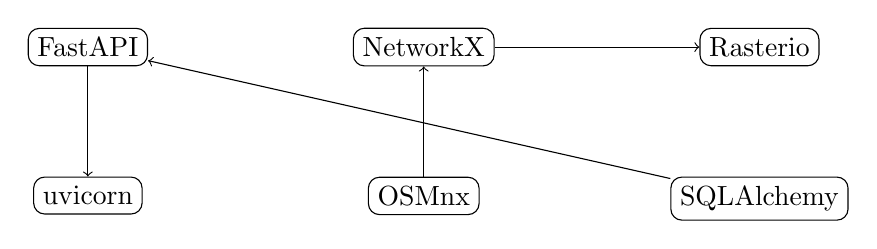
\begin{tikzpicture}[node distance=1.4cm]
    \node[draw,rounded corners] (fa) {FastAPI};
    \node[draw,rounded corners,below=of fa] (uv) {uvicorn};
    \node[draw,rounded corners,right=2.6cm of fa] (nx) {NetworkX};
    \node[draw,rounded corners,below=of nx] (ox) {OSMnx};
    \node[draw,rounded corners,right=2.6cm of nx] (rs) {Rasterio};
    \node[draw,rounded corners,below=of rs] (sa) {SQLAlchemy};
    \draw[->] (fa)--(uv);
    \draw[->] (ox)--(nx);
    \draw[->] (nx)--(rs);
    \draw[->] (sa)--(fa);
  \end{tikzpicture}
\end{frame}

\begin{frame}{Frontend Component Architecture (Sketch)}
  \small
  \begin{itemize}
    \item \texttt{MapboxMap} (GeoTIFF overlay, route layer, markers)
    \item Hooks: \texttt{useWebSocket}; Context: \texttt{WebSocketContext}
  \end{itemize}
\end{frame}

\begin{frame}{Performance Profiling (If Asked)}
  \small
  \begin{itemize}
    \item A* dominates \(\sim\)60\% CPU
    \item Memory peak \(\sim\)150MB
    \item Opportunities: bidirectional A*, heuristic tuning
  \end{itemize}
\end{frame}

\begin{frame}{Historical Flood Events Dataset (Planned)}
  \small
  \begin{tabular}{lllll}
    \toprule
    Event & Date & Max Level & Impassable Roads & Duration \\
    \midrule
    Ondoy & 2009-09-26 & 21.5m & 50+ & 12h \\
    Ulysses & 2020-11-12 & 18.2m & 30+ & 8h \\
    \bottomrule
  \end{tabular}
\end{frame}

\begin{frame}{Comparative Baseline Design (Planned)}
  \small
  \textbf{MAS-FRO (Current)}: 5 distributed agents; async collection; message-based; robust isolation.\\
  \textbf{Baseline (To Implement)}: Single process; synchronous collection; direct calls; simpler but less robust.
\end{frame}

\end{document}


